\documentclass[11pt]{article}

\usepackage[margin=1in]{geometry}
\usepackage{graphicx}
\usepackage[style=ieee,backend=biber,maxbibnames=99]{biblatex}
\usepackage{amsmath}
\usepackage{hyperref}
\usepackage{cleveref}

\title{Finding error bands for a ROC curve}
\author{Heshy Roskes}
\date{}

\newcommand{\xdot}{\dot{x}}
\newcommand{\ydot}{\dot{y}}
\newcommand{\Xdot}{\dot{X}}
\newcommand{\Ydot}{\dot{Y}}
\newcommand{\AUC}{AUC}
\begin{document}
\maketitle

\section{Introduction}

We want to solve the following problem:

We have a set of samples characterized by a parameter \(t\) (for example, density of CD8+FoxP3+-like donuts).  They are divided into two groups (responders and non-responders to anti-PD1).  We expect that one group (responders) will have a higher \(t\) than the other group (non-responders) and want to illustrate this using a ROC curve.  How can we estimate the uncertainties on the ROC curve?

One source of uncertainty is the statistics of our sample set.  We don't know the real distribution of \(t\) for the two groups; we only know the distribution for the samples we have.

Each sample's \(t\) measurement also comes with its own statistical and systematic uncertainties.  The systematic uncertainties might also be correlated between all the samples or between a subset of the samples (and this subset could include some samples from both groups).

At this point I want to address the first source of uncertainty.  I think the method will extend nicely to sample-wise uncertainties too.

\section{Previous approaches}

\section{Formalizing the problem}

\subsection{Lagrangian approach}
\label{sec:lagrangian}

A ROC curve is a plot of \(x(t), y(t)\), where \(x(t)\) is the cumulative density function (CDF) of \(t\) for one group (non-responders) and \(y(t)\) is the CDF for the other group (responders).  The derivatives, \(\xdot(t)\) and \(\ydot(t)\), give the probability density functions (PDFs) for the two groups.   We want to find a probability distribution for the ``true'' \(x\) and \(y\) distributions, given our observed data.

Our observed data for the two groups have CDFs \(X(t), Y(t)\) and PDFs \(\Xdot(t), \Ydot(t)\).  In reality \(\Xdot\) and \(\Ydot\) are going to be sums of delta functions, but for the time being we will treat them as continuous and use continuous distributions in our tests.  They are normalized so that
\begin{align}
\begin{aligned}
X(-\infty)=Y(-\infty)&=0 \\
X(+\infty)&=n_X \\
Y(+\infty)&=n_Y
\end{aligned}
\end{align}

The probability density to observe a non-responder or responder at \(t_i\) is just \(\xdot(t)\) or \(\ydot(t)\), and the log likelihood is \(\ln{\xdot(t)}\) or \(\ln{\ydot(t)}\).  Summing this log likelihood over our whole observed dataset, we get
\begin{equation}
	-2\ln{L}=-2\int_{-\infty}^{\infty}dt\left(\Xdot(t)\ln{\xdot(t)}+\Ydot(t)\ln{\ydot(t)}\right).
	\label{eq:loglikelihood}
\end{equation}
We want to find \(x(t)\) and \(y(t)\), given \(\Xdot(t)\) and \(\Ydot(t)\).  Note that we have the boundary conditions
\begin{align}
\begin{aligned}
	x(-\infty)=y(-\infty)&=0\\
	x(+\infty)=y(+\infty)&=1
\end{aligned}
\label{eq:boundaryconditions}
\end{align}

To do find \(x\) and \(y\), we minimize \cref{eq:loglikelihood}.  Our Lagrangian is
\begin{equation}
	\mathcal{L}[x,\xdot,y,\ydot,t]=-2\left(\Xdot(t)\ln{\xdot(t)}+\Ydot(t)\ln{\ydot(t)}\right),
	\label{eq:lagrangian}
\end{equation}
and the Euler-Lagrange equations are
\begin{align}
\begin{aligned}
	\frac{\partial\mathcal{L}}{\partial x}-\frac{d}{dt}\frac{\partial\mathcal{L}}{\partial \xdot}&=0 \\
	-\frac{d}{dt}\left(-2\frac{\Xdot}{\xdot}\right)&=0 \\
	\frac{\Xdot}{\xdot}&=\frac{1}{A} \\
	x&=AX+B.
\end{aligned}
\end{align}
Applying the boundary conditions, and applying the symmetric logic to \(y\), we get
\begin{align}
\begin{aligned}
	x&=X/n_X \\
	y&=Y/n_Y
\end{aligned}
\end{align}
In other words, the most likely probability distribution given our data is the probability distribution that we observe in the data.  No surprise.

\subsection{Likelihood scan for AUC}

One metric that is commonly used to assess the power of \(t\) to separate the two groups is the AUC, or area under the ROC curve.  Using our notation, this is
\begin{align}
\begin{aligned}
	\AUC&=\int_{0}^{1}ydx\\
	&=\int_{-\infty}^{\infty}y\xdot dt \label{eq:AUC}
\end{aligned}
\end{align}
We want to find a way to estimate the error on the AUC.  To do this, we will use a likelihood scan:
\begin{enumerate}
	\item Fix the AUC to a particular value
	\item Of all possible curves \(x(t), y(t)\) that satisfy \cref{eq:AUC}, find the one that is most likely given our data
	\item Plot the negative log likelihood (\cref{eq:loglikelihood}) as a function of the AUC.  The most likely AUC is the one that minimizes this log likelihood, which we found in \cref{sec:lagrangian}, and we subtract this minimum to obtain \(-2\Delta\ln{L}\).  The 68\% confidence interval is where \(-2\Delta\ln{L}<1\), and the 95\% confidence interval is where \(-2\Delta\ln{L}<3.84\).
\end{enumerate}

To minimize the log likelihood given a fixed AUC, we add a Lagrange multiplier term to the Lagrangian \cref{eq:lagrangian} to obtain
\begin{equation}
\mathcal{\tilde{L}}[x,\xdot,y,\ydot,t,\Lambda]=-2\left(\Xdot(t)\ln{\xdot(t)}+\Ydot(t)\ln{\ydot(t)}\right)+\Lambda y\xdot
\end{equation}
The Euler-Lagrange equations are:
\begin{align}
\begin{aligned}
\frac{\partial\mathcal{L}}{\partial x}-\frac{d}{dt}\frac{\partial\mathcal{L}}{\partial \xdot}&=0 \\
-\frac{d}{dt}\left(-2\frac{\Xdot}{\xdot}+\Lambda y\right)&=0 \\
2\frac{\Xdot}{\xdot}-\Lambda y&=c_1 \\
\Lambda y \xdot + c_1 \xdot - 2\Xdot&=0
\end{aligned}
\qquad
\begin{aligned}
\frac{\partial\mathcal{L}}{\partial y}-\frac{d}{dt}\frac{\partial\mathcal{L}}{\partial \ydot}&=0 \\
\Lambda \xdot-\frac{d}{dt}\left(-2\frac{\Ydot}{\ydot}\right)&=0 \\
2\frac{\Ydot}{\ydot}+\Lambda x&=c_2 \\
-\Lambda x \ydot + c_2 \ydot - 2\Ydot&=0 \\
\end{aligned}
\label{eq:eulerlagrange_AUC}
\end{align}

In addition to the boundary conditions from \cref{eq:boundaryconditions}, we also have \cref{eq:AUC}.  We can integrate the Euler-Lagrange equations \cref{eq:eulerlagrange_AUC} to obtain:
\begin{align}
\begin{aligned}
\int_{-\infty}^{\infty}dt\left(\Lambda y \xdot + c_1 \xdot - 2\Xdot\right)&=0 \\
\Lambda\AUC+c_1-2n_X&=0
\end{aligned}
\qquad
\begin{aligned}
\int_{-\infty}^{\infty}dt\left(-\Lambda x \ydot + c_2 \ydot - 2\Ydot\right)&=0 \\
-\Lambda(1-AUC)+c_2-2n_Y&=0
\end{aligned}
\label{eq:boundaryconditions_AUC}
\end{align}
We actually now have one boundary condition too many: we need five, one each for \(x\), \(y\), \(c_1\), \(c_2\) and \(\Lambda\).  One of them is redundant.

This system of differential equations can be solved using \texttt{scipy.integrate.solve\_bvp}.

\subsubsection{Example}

For the first example I tried a simple test with three events in each category: the non-responders have \(t=\left(-1, 2, 2\right)\) and the responders have \(t=\left(-2, -2, 1\right)\).  Instead of delta functions, the data distributions \(X(t)\) and \(Y(t)\) are sums of normal distributions with a width of \(0.6\).  The data distributions and ROC curve are shown in \cref{fig:exampledata}.

\begin{figure}
\begin{center}
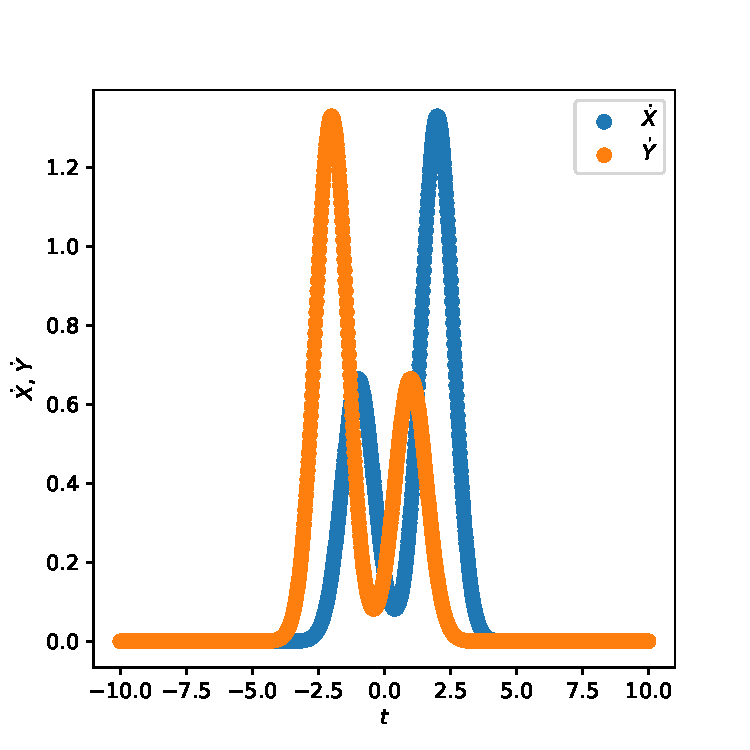
\includegraphics[width=0.32\textwidth]{exampleXdotYdot.pdf}
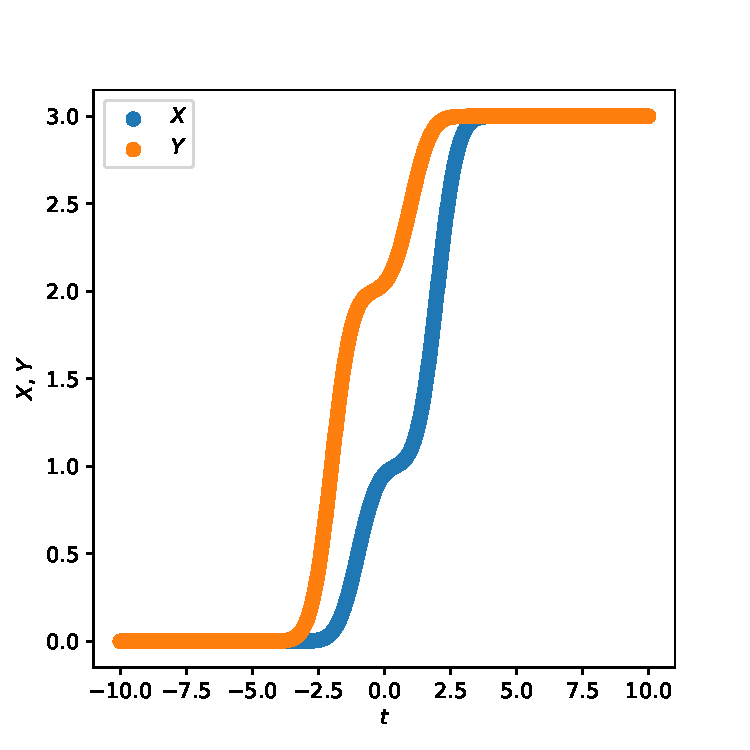
\includegraphics[width=0.32\textwidth]{exampleXY.pdf}
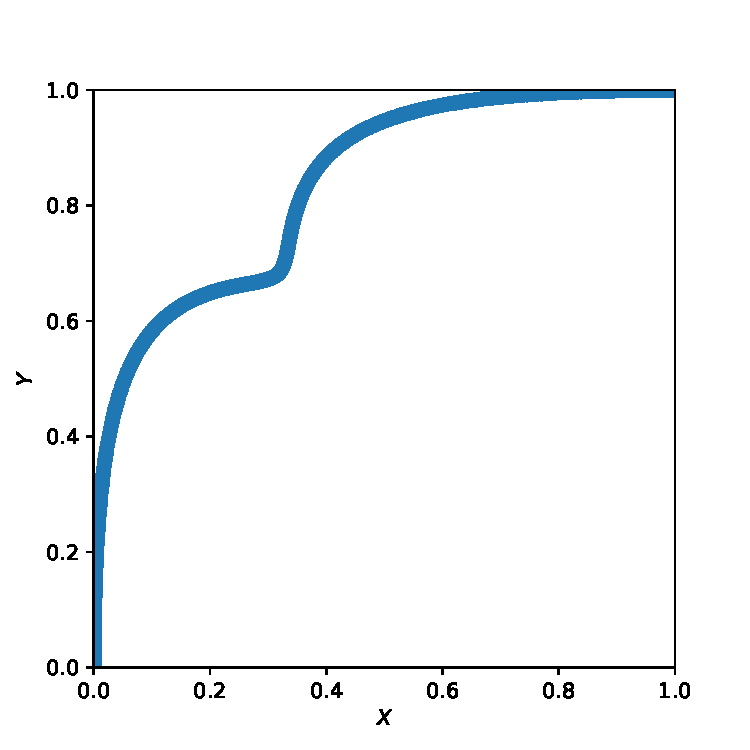
\includegraphics[width=0.32\textwidth]{exampleroc.pdf}
\caption{Plots for the example distributions.  Left: The density of non-responders \(\Xdot\) and responders \(\Ydot\).  Middle: The cumulative density of non-responders \(X\) and responders \(Y\).  Right: The ROC curve.}
\label{fig:exampledata}
\end{center}
\end{figure}

I tried plugging the differential equations \cref{eq:eulerlagrange_AUC} and boundary conditions \cref{eq:boundaryconditions,eq:boundaryconditions_AUC} into \texttt{scipy.integrate.solve\_bvp}.  For some range of \(\AUC\), this works pretty well.  I have to give it a decent starting guess for the curve and \(\Lambda\).  The way I do this is to start from the actual ROC curve (which is the solution when \(\AUC\) is the actual \(\AUC\) for \(x=X/n_X\) and \(y=Y/n_Y\)) and moving outwards in small increments.  Each time, the guess uses the fitted \(\Lambda\) and ROC curve, adjusted slightly to match the desired \(\AUC\), from the previous step.

There are two possible ways \texttt{solve\_bvp} can fail.  It can fail to converge, of course, but it can also converge on the following fake solution, which satisfies \cref{eq:eulerlagrange_AUC,eq:boundaryconditions,eq:boundaryconditions_AUC}:
\begin{align}
\begin{aligned}
x&=\Xdot/n_X \\
y&=\Ydot/n_Y \\
\Lambda&=0 \\
c_1&=2n_X \\
c_2&=2n_Y
\end{aligned}
\end{align}
In other words, \cref{eq:boundaryconditions_AUC} is a necessary but not sufficient replacement for \cref{eq:AUC}.  I'm not sure how to come up with a better boundary condition.  On the other hand, it may not matter so much, because \texttt{solve\_bvp} needs a decent guess anyway in order to converge.

A bigger issue is that beyond a certain point, \texttt{solve\_bvp} fails to converge even if I give it a guess based on an AUC that is very close by.

\end{document}